%%%%%%%%%%%%%%%%%%%%%%%%%%%%%%%%%%%%%%%%%%%%%%%%%%%%%%%%%%%%%%%%%%%%%%%%
% Preamble
%%%%%%%%%%%%%%%%%%%%%%%%%%%%%%%%%%%%%%%%%%%%%%%%%%%%%%%%%%%%%%%%%%%%%%%%
\documentclass[10pt]{article}
%
% Packages and other includes
% Pagination
\usepackage[letterpaper, margin=0.7in]{geometry}
\usepackage{emptypage}
\usepackage{ulem}
\usepackage{xcolor}
\usepackage{mhchem}
%
% Fonts
\usepackage[T1]{fontenc} % best for Western European languages
\usepackage{lmodern} % Latin Modern instead of CM
\usepackage{textcomp} % required to get special symbols
%
% Math
\usepackage{amsmath, amssymb}
\usepackage{braket}
%
% Graphics, floats, tables
\usepackage{graphicx, color, float, array}
%
% Hyperlinks
\usepackage{hyperref}
%
%
% Definitions and settings
% Paragraph indent and spacing
\setlength{\parskip}{0.4\baselineskip}
\setlength{\parindent}{0in}
%
%
% Title, authors, date
\title{\textbf{Week 9 Discussion}}
\date{\vspace{-2em}March 1st, 2022}
%
%
%%%%%%%%%%%%%%%%%%%%%%%%%%%%%%%%%%%%%%%%%%%%%%%%%%%%%%%%%%%%%%%%%%%%%%%%
% Main document
%%%%%%%%%%%%%%%%%%%%%%%%%%%%%%%%%%%%%%%%%%%%%%%%%%%%%%%%%%%%%%%%%%%%%%%%
%

\begin{document}

\maketitle

1. \textbf{State Change of an Ideal Gas} 1.50 mol of N$_2$ gas at a constant
pressure of 1.50 atm is allowed to expand from 8.00 L to 15.00 L accompanied
by a temperature change from 97.5 K to 183 K. Assume ideal gas conditions.

(a) Estimate C$_{P,m}$ using the equipartition theorem.

(b) Compute the change in enthalpy for this state change.

2. \textbf{Equipartition Theorem} 2.150 mol of CH$_4$(g) at a constant volume
of 1.00 L is heated from 220 K to 260 K accompanied by an increase in pressure
from 15.4 bar to 28.1 bar. Assume ideal gas conditions.

(a) Estimate C$_{V,m}$ using the partition theorem.

(b) Compute the change of internal energy for this state change.

3. \textbf{Van't Hoff Equation} Ca(OH)$_2$(aq) is a sparingly soluble ionic salt. The
temperature dependence of the solubiility product constant $K_{sp} = \text{a(Ca$^{2+}$)
  a$^2$(OH$^-$)$_2$}$ of Ca(OH)$_2$(aq) is plotted below

\begin{figure}[hbpt]
  \centering
  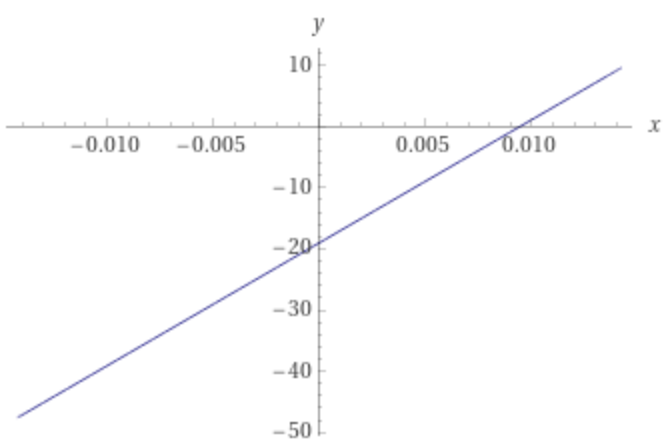
\includegraphics[scale=0.3]{vant_hoff.png}
  \caption{Van't Hoff plot with the form $y = 2010.9x - 10.002$.}
\end{figure}

(a) Using the linear regression from the plot above, determine the standard molar enthalpy
and entropy for the dissolution of Ca(OH)$_2$(aq).

(b) If the temperature is decreased, does the solubility of Ca(OH)$_2$(aq) increase,
decrease or stay the same?

4. \textbf{Thermodynamic Equilibrium} A chemist needs to prepare the compound PH$_3$BCl$_3$(s)
according to the following reaction for which $K = 19.2$ at 50.0$^\circ$C.

\begin{center}
  PH$_3$(g) + BH$_3$(g) $\rightleftharpoons$ PH$_3$BH$_3$(s)
\end{center}

\begin{table}[hbpt]
  \centering
  \begin{tabular}{c|c}
    Molecule & $\Delta H^\circ_f$ (kJ/mol) \\
    \hline
    PH$_3$(g) & 5.47   \\
    BH$_3$(g) & 106.69 \\
    PH$_3$BH$_3$(s) & 3.55
  \end{tabular}
  \caption{$\Delta H^\circ_f$ for various compounds.}
\end{table}

(a) Determine the equilibrium constant $K$ at $70.0^\circ$C.

(b) Determine the standard molar free energy of reaction at $50.0^\circ$C.

\end{document}
